\documentclass[12pt]{article}
\usepackage[utf8]{inputenc}
%\usepackage[margin=1in]{geometry}
\usepackage{amssymb}
\usepackage{amsmath}
\usepackage{mathtools}
\usepackage{amsthm}
\usepackage{setspace}
\usepackage{cancel}
\usepackage{bbm}
\usepackage{pgfplots}
\usepackage{listings}
\usepackage{float}
\usepackage{hyperref}

\usetikzlibrary{arrows, calc, patterns, shapes}
  \pgfplotsset{compat=1.15}
\renewcommand{\baselinestretch}{1.25}
\newcommand\sbullet[1][.5]{\mathbin{\vcenter{\hbox{\scalebox{#1}{$\bullet$}}}}}
\newcommand{\indep}{\perp \hspace{-.5 em} \perp}
\def\E{\mathbb{E}}
\def\e{\mathcal{E}}
\def\d{\mathcal{D}}
\def\I{I_n}
\def\l{\ell}
\def\sumn{\sum^n_{i=1}}
\def\i{\mathcal{J}}
\def\x{\mathbf{X}}
\def\inv{^{-1}}
\def\f{Fréchet }
\newcommand{\til}[1]{\underset{\sim}{#1}}
\newcommand\expp[1]{\exp\bigg\{#1\bigg\}}
\newcommand\der[2]{\frac{\partial #1}{\partial #2}}
\newcommand{\ds}{\displaystyle}
\lstset{frame=tb,
  language=Python,
  aboveskip=3mm,
  belowskip=3mm,
  showstringspaces=false,
  columns=flexible,
  basicstyle={\small\ttfamily},
  numbers=none,
  numberstyle=\tiny\color{gray},
  keywordstyle=\color{blue},
  commentstyle=\color{red},
  stringstyle=\color{mauve},
  breaklines=true,
  breakatwhitespace=true,
  tabsize=3
}
\theoremstyle{definition}
\newtheorem{theorem}{Theorem}

\theoremstyle{definition}
\newtheorem{definition}{Definition}

\newtheorem{example}{Example}[section]

\let\inf\infty
\title{Math 80622A Final Report}
\author{Jean-Yves Djamen }
\date{Fall 2020}

\begin{document}

\maketitle
\tableofcontents{}
\doublespacing

\pagebreak


\section{Preface}
Statistical extreme value theory is a popular toolbox used in the modeling of infrequent (or extreme) events. It has been shown to be effective at several tasks, from the analysis of weather patterns \cite{test1} to financial stocks \cite{test2}. One tool in this toolbox is the generalized Pareto distribution which is used to model exceedences of data over a set threshold. While this tool is popular, there are practical difficulties that may arise when trying to find an appropriate threshold over which to fit data. In their work, \cite{papatawn} Jonathan Tawn and Ioannis Papastathopoulos propose a new class of models to extend the generalized Pareto distribution and mitigate the practical difficulties encountered from its use. In this report, reproduction of their analyses will be conducted alongside new analysis using the extended model on new data. 

\section{Generalized Pareto Model}
Given a random variables, $X$, with cummulative distribution function (cdf) $F_X$ and $u_F$ defined as $u_F= \sup\{x: F_X(x)<1\}$ there is  a limiting result \cite{gpd} for the conditional distribution $X-u|X>u$: 
\[ \lim_{u\rightarrow u_F }P(X-u < y|X>u) = 1-\bigg( 1+ \frac{\xi y}{\sigma}\bigg)^{-1/\xi} \tag{1}\]
Where (1) is the cdf of a generalized Pareto (GP) distribution with parameters $\sigma$ as the scale and $\xi$ as the tail index. Once this result holds for a threshold $u<u_F$, it will hold for all thresholds $u'>u$. As previously mentioned, finding an appropriate threshold $u$ to use in practice can be a challenging problem. A standard practice for threshold selection consists of fitting GP models over a range of thresholds, then plotting the modified scale ($\sigma^*$) defined below over a varying range of thresholds. The minimum threshold after which $\sigma^*$ stabilizes is then chosen as the threshold.
\[\sigma^*= \sigma_u-\xi u\]
In practice, such a threshold may not exist or may be too large relative to the data at hand. Large thresholds result in loss of data and high variance in the estimated parameters. For this reason, \cite{papatawn} proposes 3 new models to serve as extensions to the GP distribution. 

\section{Extended Generalized Pareto Models}
Let $U\sim \mathcal{U}(0,1)$ be a uniform random variable defined on (0,1) and let $G$ be the cdf of a GP$(\sigma,\xi)$. Then, by standard statistical calculations (probability integral transform) the new random variable defined as $V=G^{-1}(U)$ also follows a GP distribution. To form their extended models, \cite{papatawn} use a similar logic. This extension mechanism makes use of a pseudo probability integral transform $V=G^{-1}(Y)$ where $G$ is as before and $Y$ is a single parameter random variable with support on the unit interval. With the appropriate choice of distribution $Y$, the random variable $V$ will follow distribution EGP$(\kappa, \sigma,\xi)$ where $\xi$ is conserved as the tail index \cite{papatawn}. An additional constraint for the choice of $Y$ is to get a resulting random variable $V$ such that, for a specific value $\kappa^*$, EGP$(\kappa^*, \sigma,\xi)$=GP$(\sigma,\xi)$ thus connecting the base distribution to the proposed extensions. 

\subsection{Extended Distributions}
As this report is not meant to reproduce $\cite{papatawn}$, this section serves only as a place to define the proposed models for later reference. First, the probability density function of the three models  arising from the extension mechanism discussed above.
\footnote{Be denotes the beta function}

\begin{align*}
g_{EGP1}(x,\kappa,\sigma,\xi)&=\begin{cases} \frac{|\xi|/\sigma}{\text{Be}(\kappa, |\xi|^{-1})}\{1-(1+\xi x/\sigma)_+^{-|\xi|/\xi}\}^{\kappa-1} (1+\xi x/\sigma)_+^{-1/\xi-1} & \xi \neq 0\\\\
    \frac{\sigma^{-1}}{\Gamma(\kappa)}x^{\kappa-1}e^{-x/\sigma} & \xi \rightarrow 0
    \end{cases}\\
    g_{EGP2}(x,\kappa,\sigma,\xi)&= \begin{cases}\frac{\sigma^{-1}}{\Gamma(\kappa)}\{\xi^{-1}\log(1+\xi x/\sigma)_+\}^{\kappa-1} (1+\xi x/\sigma)_+^{-1/\xi-1} & \xi\neq 0\\\\
    \frac{\sigma^{-1}}{\Gamma(\kappa)}x^{\kappa-1}e^{-x/\sigma} & \xi\rightarrow 0
    \end{cases}
\end{align*}
\begin{align*}
    g_{EGP3}(x,\kappa,\sigma,\xi)&= \begin{cases} \frac{\kappa}{\sigma}\{1-(1+\xi x/\sigma)^{\kappa-1}(1+\xi x/\sigma)_+^{-1/\xi-1}\} & \xi \neq 0\\\\
    \frac{\kappa}{\sigma}(1-e^{-x/\sigma})^{\kappa-1}e^{-x/\sigma} & \xi \rightarrow 0
    \end{cases}
\end{align*}
Next, the corresponding likelihood functions used to estimate parameters from the fit of these models to data. Given a random sample $\boldsymbol x$ of $n_u$ exceedences over $u$, the corresponding model likelihoods are given as follows:
\begin{align*}
    \ell^{EGP1}(\kappa, \sigma,\xi|\boldsymbol{x})=&n_u\log\bigg\{ \frac{|\xi|/\sigma} {Be(\kappa, |\xi|^{-1}}\bigg\}+(\kappa-1)\sum_{i=1}^{n_u}\log[1-\{1+\xi(x_i-u)/\sigma\}_+^{-|\xi|/\xi}]\\
    &-(1/\xi+1)\sum_{i=1}^{n_u}\log\{1+\xi(x_i-u)/\sigma\}_+\\
    \ell^{EGP2}(\kappa, \sigma,\xi|\boldsymbol{x})=&n_u\log\bigg\{ \frac{\sigma^{-1}}{\Gamma(\kappa)}\bigg\}+(\kappa-1)\sum_{i=1}^{n_u}\log[\xi^{-1}\log\{1_\xi(x_i-u)/\sigma\}_+]\\
    &-(1/\xi+1)\sum_{i=1}^{n_u}\log\{1+\xi(x_i-u)/\sigma\}_+\\
    \ell^{EGP3}(\kappa, \sigma,\xi|\boldsymbol{x})=&n_u\log(\kappa/\sigma)+(\kappa-1)\sum_{i=1}^{n_u}\log[1-\{1+\xi(x_i-u)/\sigma\}_+^{-1/\xi}]\\
    &-(1/\xi+1)\sum_{i=1}^{n_u}\log\{1+\xi(x_i-u)/\sigma\}_+
\end{align*}
Finally, given the probability of an exceedance $\zeta_u$, the $T$-observation return levels can be computed. \footnote{$\gamma^{-1}, \beta^{-1}$ are the inverses of the incomplete gamma and beta functions respectively}
\begin{align*}
    x_T^{EGP1}&= u + \frac{\sigma}{\xi} [\{1-\beta^{-1}(1-(T\zeta_u)^{-1},\kappa, |\xi|^{-1})\}{\-\xi/|\xi|}-1]\\
    x_T^{EGP2}&= u + \frac{\sigma}{\xi} [\exp\{\xi\gamma^{-1}(\kappa,1-(T\zeta_u)^{-1})\}-1]\\
    x_T^{EGP3}&= u + \frac{\sigma}{\xi}[\{1-(1-(T\zeta_u)^{-1/\kappa})\}^{-\xi}-1]
\end{align*}

\subsection{Extension to Available Tools }
In the proposal of these extended generalized Pareto (EGP) models, \cite{papatawn} gives plenty of motivation for the use of EGPs in conjunction to the standard GP. First, the increased flexibility of EGPs induced by parameter $\kappa$ may allow the fitting of EGPs over a lower threshold than can be fitted over a GP. This could yield models with more reliability and statistical power as they utilize more data. Additionally, since EGP(1,$\sigma,\xi$)=GP$(\sigma,\xi$), the EGPs can produce more diagnostics for the GP distribution \cite{papatawn}. Parameter stability plots from an EGP fit along varying thresholds could disseminate information on the GP model. Examining these plots, and selecting the minimum threshold after which $\kappa$ is not significantly different from 1 and the modified scale and tail index are constant could yield the threshold value after which the EGP can be simplified to the GP. Though not excessively discussed in \cite{papatawn} this method could provide a correspondence between EGPs and GP models. This correspondence is explored in both the reproduced and novel set of experiments.


\section{Simulation Study}
In the simulation study from \cite{papatawn}, 10000 samples of size $n=100,1000, 10000$ data points generated from a distribution $\mathcal{D}$. For $\mathcal{D}$, the distributions used are Normal(0,1), Student's $t_2$, and Beta(1.5,3) motivated by \cite{papatawn} as representing three domains of attraction $\xi<0, \xi=0, \xi>0$ respectively. The first criticism of \cite{papatawn} comes from its formulation of this simulation. The tail index assignment is false as calculations from \cite{index} indicate. Nevertheless, for each sample, an EGP1, EGP2 and GP model is fit over a range of equally spaced thresholds. The root mean square error for estimating the $T_1, T_2$ \footnote{$T_1=n*1.5 , T_2=n*5$} observation return level is compared across models. In the reproduction of this experiment, the sample size is reduced from 10000 to 250. 

Due to this reduced number of samples, some observations in \cite{papatawn} were unable to be reproduced. Primarily amongst these is the observation that the distance between the optimal threshold (where minimum RMSE occurs) for the EGP1 and GP gets smaller as $n$ grows. Table 1 depicts the optimal thresholds for estimation of return levels of each sample size. From this table, it is apparent that the distance between the RMSE from the EGP1 and GP model from the reproduction experiment does not decrease as size increase.

\begin{table}[H]
    \centering
    \begin{tabular}{||c|c|c|c||}\hline
\multicolumn{4}{||c||}{$T_1$}\\\hline\hline
    Model& $n=100$& $n=1000$& $n=10000$\\\hline
    $u_{EGP}$ & -2.5(-2.32)& -0.23 (0.05) & 0.09(1.48)  \\
     $u_{GP}$& -2.5 (-0.33) & -2.5 (0.45) & -0.067(1.70)\\\hline\hline
     \multicolumn{4}{||c||}{$T_2$}\\\hline\hline
     $u_{EGP}$ & -2.5(-2.32)& -0.163 (0.51) & 0.492(1.44)  \\
     $u_{GP}$& -2.5 (-0.23) & -0.0049 (0.68) & 0.305(1.44)\\\hline
\end{tabular}
    \caption{Optimal Threshold for estimation of long and short term return levels for each sample size. In parenthesis are the original values from \cite{papatawn}. }
\end{table}

However, a comparison of Fig. 1 (original experiment) and Fig. 2 (reproduction) shows some consistency of results across studies. The consistent conclusion being, with smaller data size $(n=100)$, the EGPs perform better than the GP models. In fact, with $n=100$, the EGP1 model performs best when fit to on exceedences over the smallest possible threshold thus highlighting the advantage of fitting EGPs (rather than GPs) when working with smaller datasets.

\begin{figure}[H]
\begin{center}
{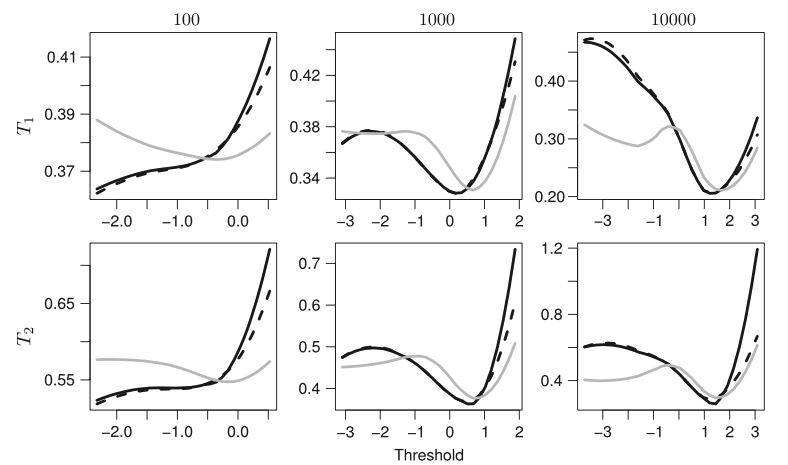
\includegraphics[width=4.0in]{project/papafiles/fig2.papa.png}}
\caption{RMSE for the $T_1$(top row) and $T_2$(bottom row) return level estimates from EGP1(black), EGP2(dashed) and GP (gray) from experiment in \cite{papatawn} with standard normal data.}
\end{center}
\end{figure}
\begin{figure}[H]
\begin{center}
{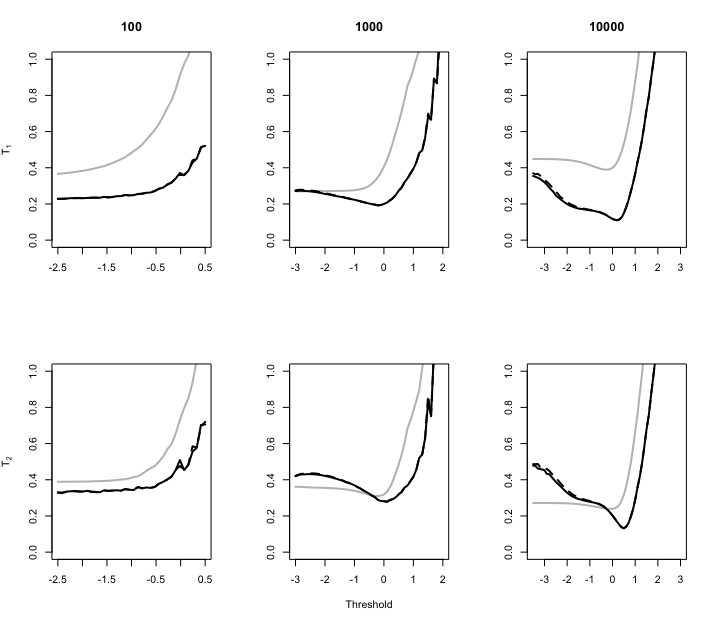
\includegraphics[width=4.0in]{project/papafiles/fig2.me.png}}
\caption{RMSE for the $T_1$(top row) and $T_2$(bottom row) return level estimates from EGP1(black), EGP2(dashed) and GP (gray) from experiment reproduction.}
\end{center}
\end{figure}
Recall that one of the proposed applications of EGP models was as a diagnostic tool for GPs through observation of estimated $\kappa$ values plotted against varying thresholds. In Fig. 3, this diagnostic tool is depicted. Similarly to the analysis in \cite{papatawn} the reproduced experiments show that the threshold for which the value 1 is inside the confidence interval for $\kappa$ corresponds (approximately) to the threshold that yields the minimum RMSE with the GP model. It should be noted that this is slightly less accurate for small samples sizes ($n=100$) in both the original and reproduction experiments.

\begin{figure}[H]
\begin{center}
{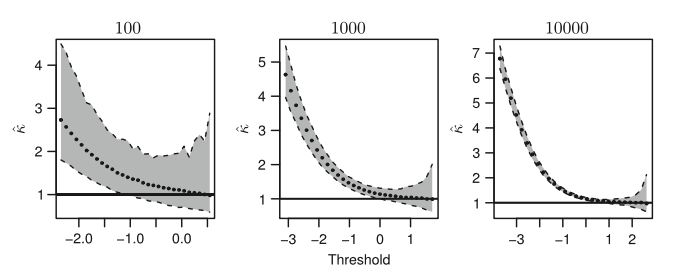
\includegraphics[width=4.0in]{project/papafiles/fig3.papa.png}}
{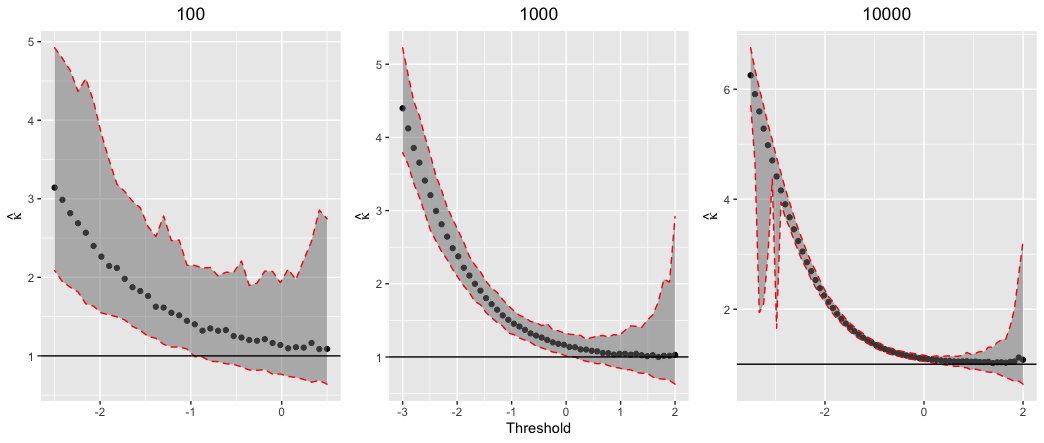
\includegraphics[width=4.0in]{project/papafiles/fig3.me.png}}
\caption{Median Monte Carlo estimates of $\kappa$ parameter plotted against each threshold for each sample size along with the 95\% Monte Carlo confidence intervals (grey). Original experiment from \cite{papatawn}(top) and reproduced experiment (bottom). }
\end{center}
\end{figure}

While the discussion so far has been focused on the simulation with standard normal data, Fig. 4 and Fig. 5 show the RMSE output of the simulation studies (original and reproduction respectively) with the other distributions. From these, the conclusions are the same: the EGP models perform better than the GP for T-observation return level inference.
\begin{figure}[H]
\begin{center}
{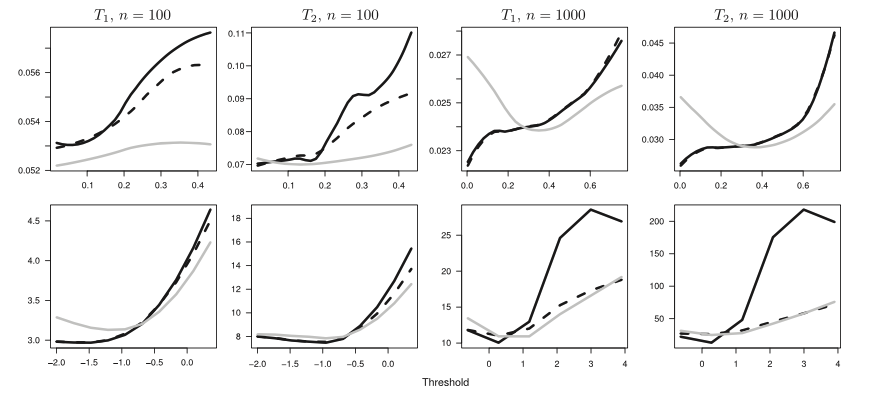
\includegraphics[width=4.0in]{project/papafiles/fig4.papa.png}}
\caption{RMSE for the $T_1$(top row) and $T_2$(bottom row) return level estimates from EGP1(black), EGP2(dashed) and GP (gray) from \cite{papatawn} simulation. First row corresponds to Beta(1.5,3) and the second to Student's $t_2$ data.}
{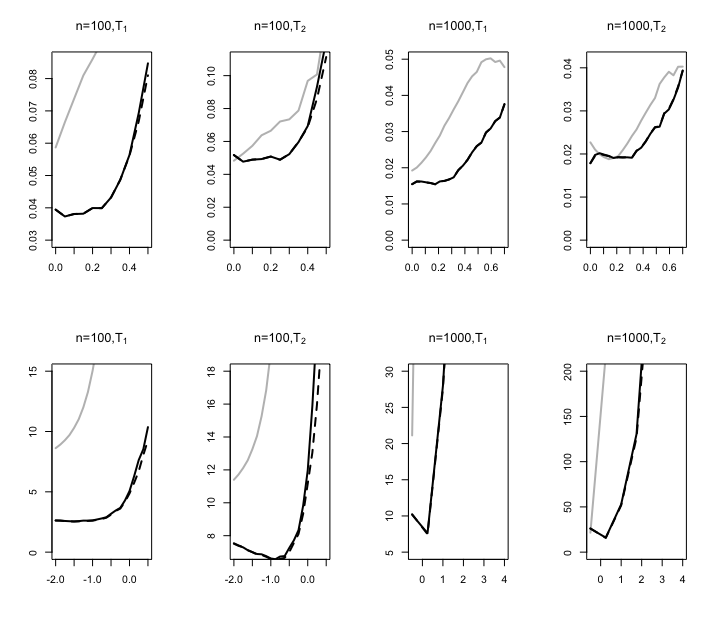
\includegraphics[width=4.0in]{project/papafiles/fig4.me.png}}
\caption{RMSE for the $T_1$(top row) and $T_2$(bottom row) return level estimates from EGP1(black), EGP2(dashed) and GP (gray) from reproduced simulation. First row corresponds to Beta(1.5,3) and the second to Student's $t_2$ data.}
\end{center}
\end{figure}



\section{Application to River Nidd Data}
This experiment uses the 154 exceedences over the threshold 65.08 $m^3/s$ of the flow of the river Nidd gathered from 1934 to 1969. In this analysis, \cite{papatawn} fits an EGP1 and a GP over a range of threshold (of length 40) varying from 65.08 to 88.61. The purpose of this analysis is three fold. First, to display the ability of the EGP1 model to perform competitively against the GP while using a lower threshold. Second, to underline the diagnostic ability of EGP1 for GP models through threshold selection. Finally, to illustrate the return level stability unique to the EGP. Though this experiment was not perfectly reproduced, sections 5.1-5.2 discuss its intent and addresses new conclusions from the reproduced experiment. 

\subsection{Selection Lower Thresholds}
First, \cite{papatawn} aim to demonstrate that the extensions to the GP can be fitted over smaller thresholds (and thus include more data) than the GP model while having similar stability in parameters estimates. From the parameter stability graphs (Fig. 6), the threshold $u=65.08$ is chosen for the EGP1 model as estimates for $\hat \kappa, \hat \sigma^*, \hat \xi$ are relatively stable past this threshold (compared to GP model).  However, the parameter stability graphs when reproducing the experiment (Fig. 7) support the choice of GP model over EGP1 as the parameters from a GP model are more stable over different thresholds. In fact, the high variability of the EGP1 estimates over different thresholds would detract some from using this method. 
\begin{figure}[H]
\begin{center}
{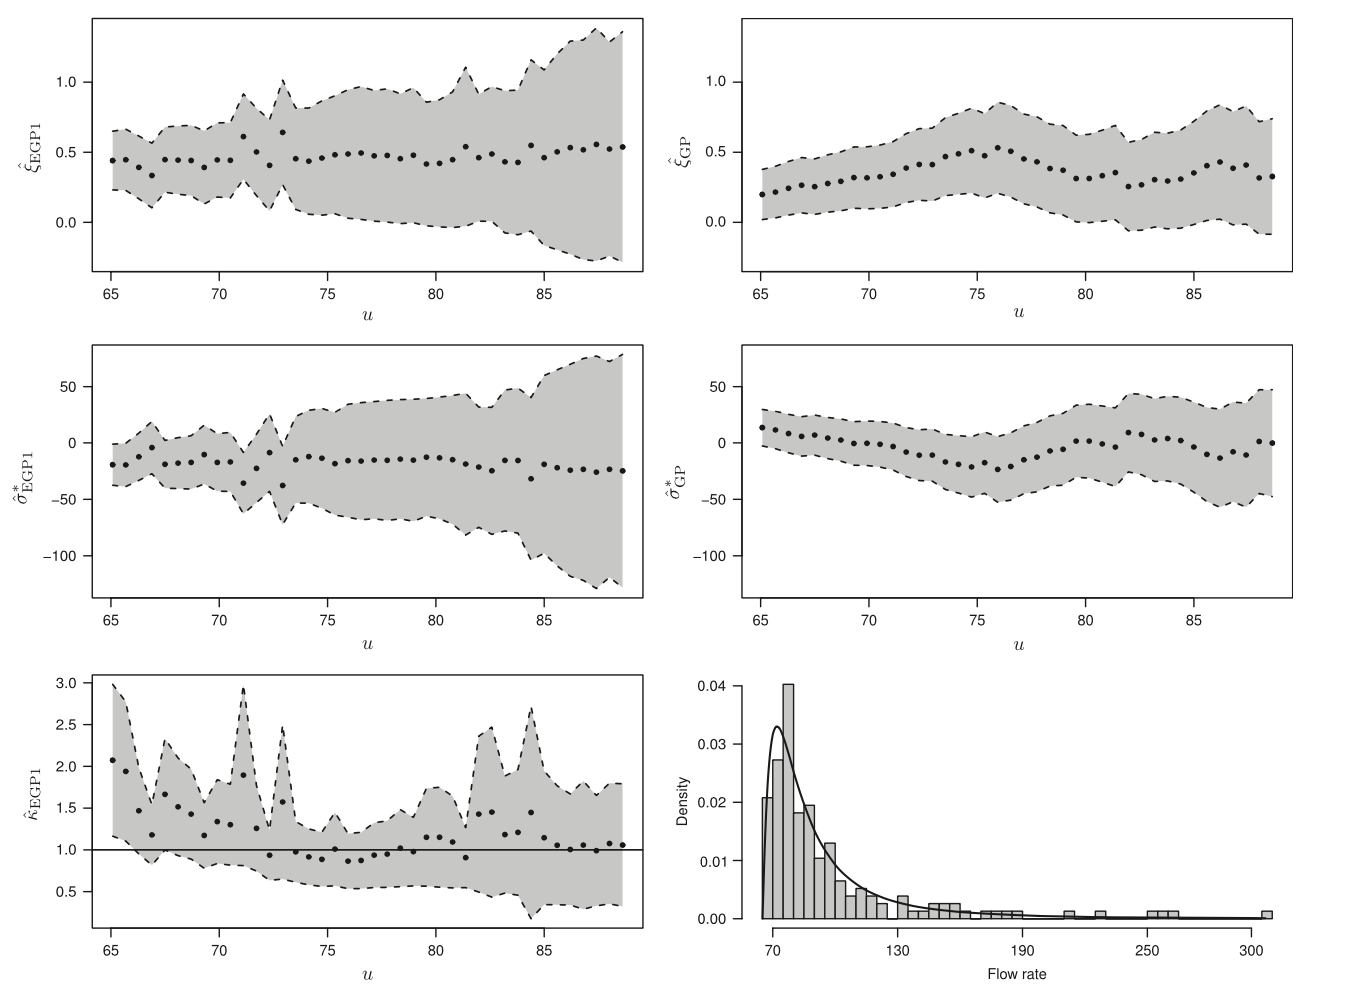
\includegraphics[width=5.0in]{project/papafiles/fig5 papa.png}}
\caption{Maximum likelihood estimates of parameters from experiment by \cite{papatawn} with 95\% confidence intervals from fitting EGP1 (left column) and GP (right column). The bottom right graph shows histogram of river Nidd data overlaid with EGP1 fitted model with $u=65.08$.}
\end{center}
\end{figure}

\begin{figure}[H]
\begin{center}
{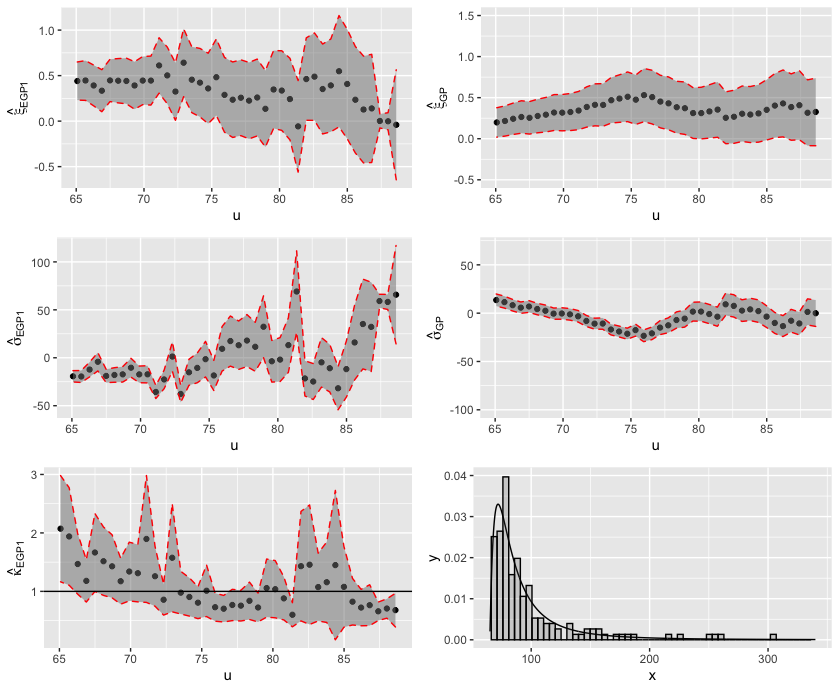
\includegraphics[width=5.0in]{project/papafiles/fig5.me.png}}
\caption{Maximum likelihood estimates of parameters from reproduction with 95\% confidence intervals from fitting EGP1 (left column) and GP (right column). The bottom right graph shows histogram of river Nidd data overlaid with EGP1 fitted model with $u=65.08$.}
\end{center}
\end{figure}

Although the parameter stability estimate conclusions are different between the experiments done here and in \cite{papatawn}, the conclusions from using the EGP1 as a diagnostic tool for the GP model are the same. Following the stability analysis, \cite{papatawn} observe that the minimum value $u$ for which $\hat\kappa$ is not significantly different from 1 is $75.3$ and remark that this choice of threshold consistent with the threshold resulting from a different analysis \cite{fig5} and thus use $u=75.3$ for the GP. Similarly, in the reproduction experiment, one of the lowest values for which $\hat\kappa$ is 75.33. 

\subsection{EGP1 Return Level Stability}
In the final experiment with the river Nidd data, \cite{papatawn} examine the stability of return level estimates from both an EGP1 and GP model. This is done through the investigation of estimated of return levels by an EGP1 and GP model over different thresholds. Fig. 8 (EGP1) and Fig. 9 (GP) are the return level stability plots for the EGP1 and GP model from the original analysis and its reproduction. Again, there are differences in the produced graphs. From the reproduction analysis, it appears that the GP estimates are more stable than the EGP estimates. This agrees with the reproduction graphs show in Fig. 7 as the GP parameter estimates seem more stable than those of the EGP1. Additionally, according to the reproduction experiments, return level estimates from neither the EGP1 nor the GP model grow with the choice of threshold.
\begin{figure}[H]
\begin{center}
{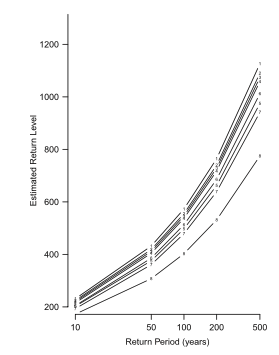
\includegraphics[width=2.0in]{project/papafiles/fig6.papa.egp1.png}}
{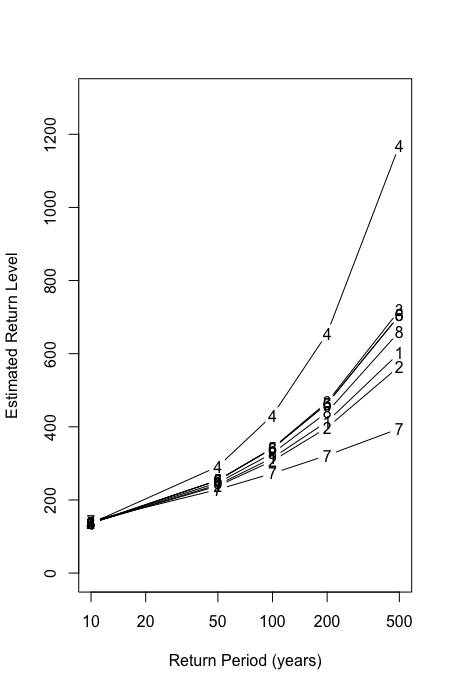
\includegraphics[width=2.0in]{project/papafiles/fig6.me.egp1.png}}
\caption{Estimates of 10-, 50-, 100-, 200- and 500-observation return level obtained from fitted EGP1 above the range of thresholds [65.08,82.6] coded here by numbers 1-8, respectively. Results from \cite{papatawn} on the left and those experiment reproduction on the right.}
\end{center}
\end{figure}
\begin{figure}[H]
\begin{center}
{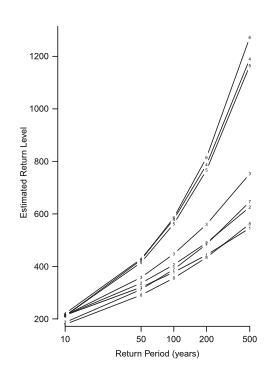
\includegraphics[width=2.0in]{project/papafiles/fig6.papa.gp.png}}
{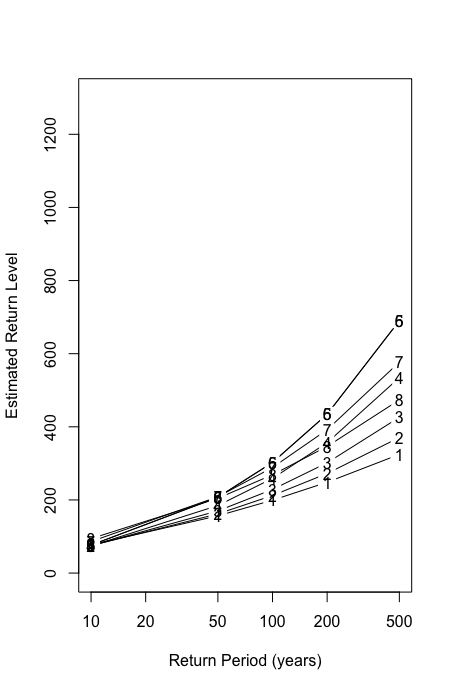
\includegraphics[width=2.0in]{project/papafiles/fig6.me.gp.png}}
\caption{Estimates of 10-, 50-, 100-, 200- and 500-observation return level obtained from fitted GP above the range of thresholds [65.08,82.6] coded here by numbers 1-8, respectively. Results from \cite{papatawn} on the left and those experiment reproduction on the right.}
\end{center}
\end{figure}
\subsection{Nidd Experiment Criticisms}
There are a few valid criticisms of the Nidd data experiments as performed by \cite{papatawn}. First, since there are no diagnostic plots shown for either the EGP1 or the GP models, the efficacy of one over the other is difficult to quantify. While the EGP1 in Fig. 6 may seem to have stable estimated parameters over varying thresholds, a quantile-quantile(qq) plot or probability-probability(pp) plot would give more information about the statistical power of the EGP1 model in comparison to the GP. QQ plots would additionally be helpful when assessing return level in Fig. 8 and Fig. 9 as they could provide a measure of accuracy.

Additionally, when finding the minimum $u$ for which $\hat \kappa$ is close to 1, it seems \cite{papatawn} chose 75.3 over 73.5. In fact, from Fig.6, it can be seen that there are 3 potential points on the interval (70,75) which could have been chosen. The choice by \cite{papatawn} seems to have been made to ensure that the results from this experiment agree with those in \cite{fig5}.

\section{Application to Pharmaceutical Data}
In this final experiment with EGPs, \cite{papatawn} investigate the relation between medication doses (labeled A, B, C, D) and liver toxicity as measured by levels of bilirubin\footnote{Biomarker for liver toxicity}. The data used consists of the residuals from linear median regression of measures of bilirubin in 606 clinical patients before and after treatment.
\begin{figure}[H]
\begin{center}
{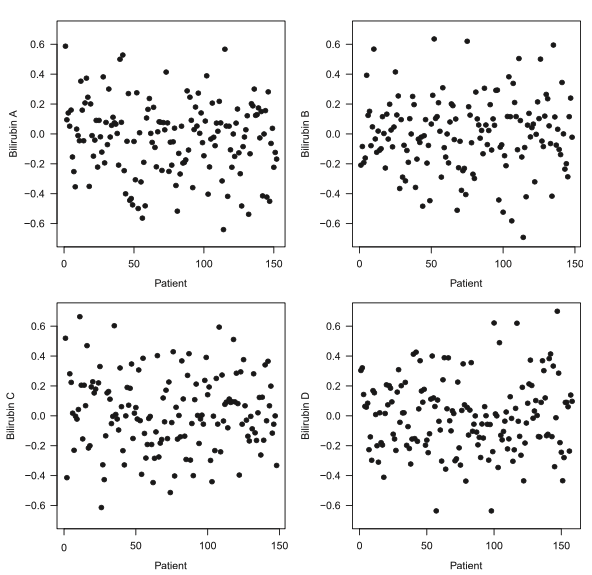
\includegraphics[width=3in]{project/papafiles/fig1.papa.png}}
{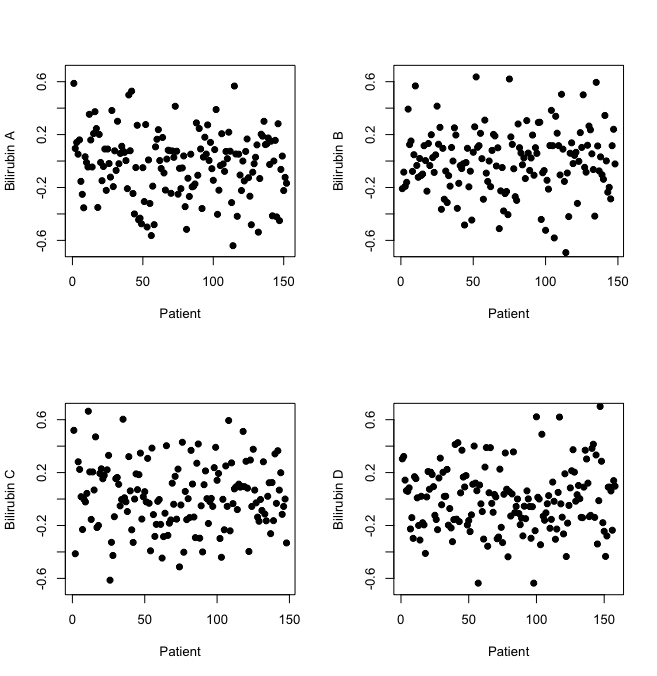
\includegraphics[width=3in]{project/papafiles/fig1.me.png}}
\caption{Residual total bilirubin after linear median regression of bilirubin concentration post-treatment on bilirubin concentration pre-treatment  from 606 patients with given medicine labeled as dose A, B, C, D. First two rows are data as shown by \cite{papatawn} and last two are data for reproduction experiment.}
\end{center}
\end{figure}

%A driving force for this experiment is the hypothesis that EGP1 models can be fit over more data points than GPs. 
Using the likelihood ratio test, \cite{papatawn} explore whether or not a model fit on the pharmaceutical data requires dose dependent parameters. First, separate EGP1 models are fit for each dose over a range of thresholds. Then, an EGP1 model is fit on the entire data with the constraint that the parameter $\hat\kappa$ is the same for different doses. Parameters $\hat \xi, \hat\sigma$ are free to differ from dose to dose.  Fig. 11 displays the estimated values of $\hat\kappa$ of such a fit over different thresholds. Finally, an EGP1 model is fit on the entire data with the constraint that both  are common across doses. The scale parameter is free to differ from dose to dose. Fig. 12 displays the change of the tail index parameter $\hat \xi$ in such a pooling scenario. As visible from the figures below, the pooled parameters were reproduced exactly. Furthermore, while the estimate dose-dependent parameters slightly differ from the originals presented by \cite{papatawn} the conclusions of the likelihood ratio test are the same.


\begin{figure}[H]
\begin{center}
{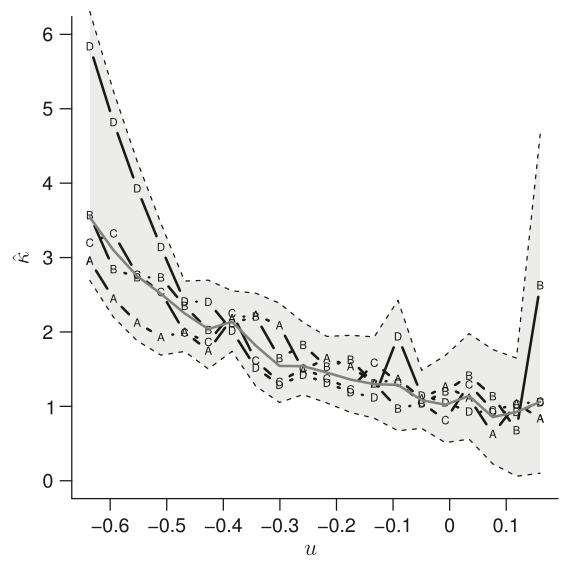
\includegraphics[width=2.0in]{project/papafiles/fig7.kap.papa.png}}
{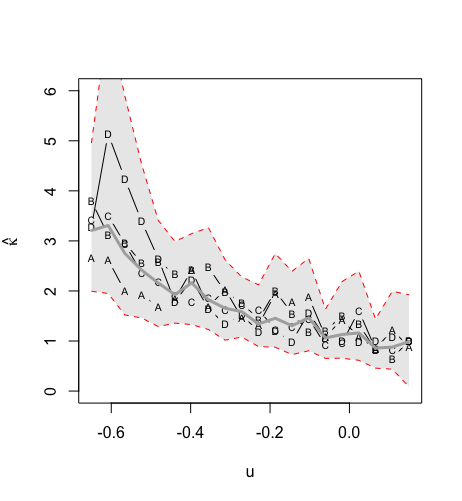
\includegraphics[width=2.0in]{project/papafiles/fig7.kap.me.png}}
\caption{Estimate of $\hat\kappa$ for dose levels $A-D$ (appropriately labeled) and  under assumption of common $\hat\kappa$ (but varying scale and tail index) parameters across doses (in grey). On the left are results from \cite{papatawn}, and on the right, results from reproduction experiment.}
{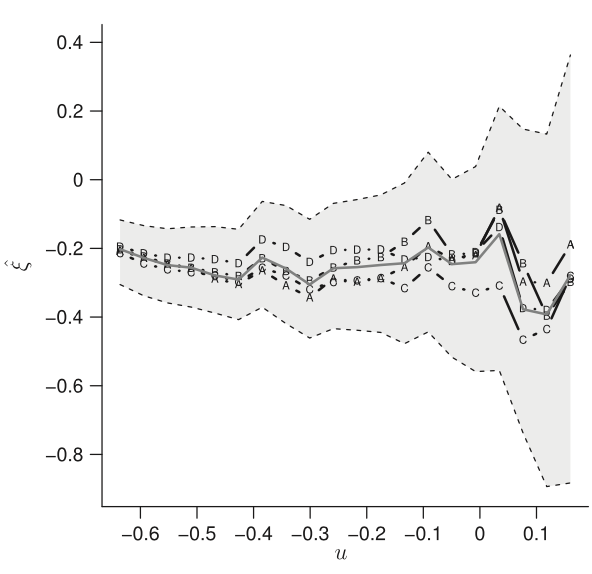
\includegraphics[width=2.0in]{project/papafiles/fig7.xi.papa.png}}
{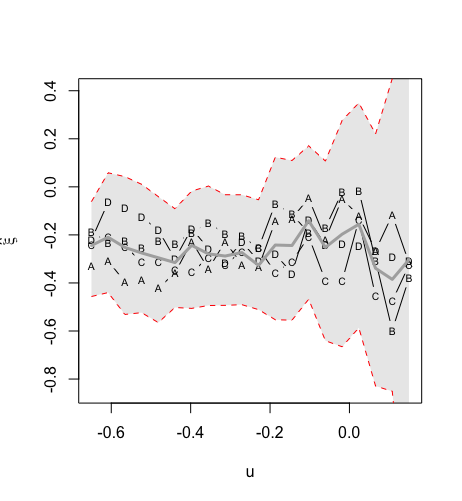
\includegraphics[width=2.0in]{project/papafiles/fig7.xi.me.png}}
\caption{Estimate of $\hat\xi$ for dose levels $A-D$ (appropriately labeled) and  under assumption of common $\hat\xi, \hat{kappa}$ (but varying scale) parameters across doses (in grey). On the left are results from \cite{papatawn}, and on the right, results from reproduction experiment.}
\end{center}
\end{figure}

The terminal step of the experiment consists of diagnostic plots for and EGP1 model fit over the 30\% quantile of the data and a GP fit over the 70\% quantile. The aim of these diagnostic plots is to reinforce the EGP1 model as an alternative to the GP model as, in this instance, it can be fit to more data points without sacrificing statistical power or increasing standard errors of estimated parameters. As can be seen by Fig. 13 and Fig. 14, the EGP1 model is utilizes much more data than the GP. Furthermore, as this EGP1 model has an estimated value of $\hat\kappa$ significantly different from 1, there is evidence that a GP model is not sufficient to model data at such a low threshold.

\begin{figure}[H]
\begin{center}
{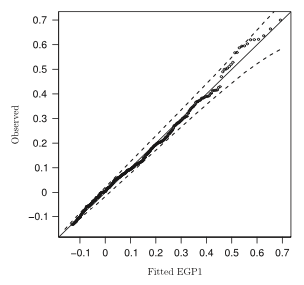
\includegraphics[width=2.0in]{project/papafiles/fig8.papa.egp1.png}}
{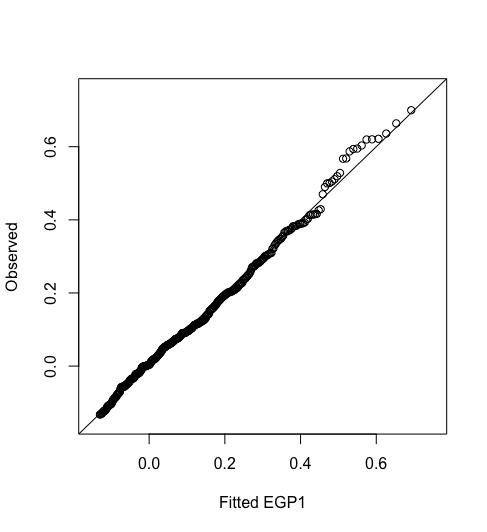
\includegraphics[width=2.0in]{project/papafiles/fig8.me.egp1.png}}
\caption{QQ plot for diagnosis of EGP1 fit of data above 30\% quantile. Left: \cite{papatawn}, right: reproduction }
{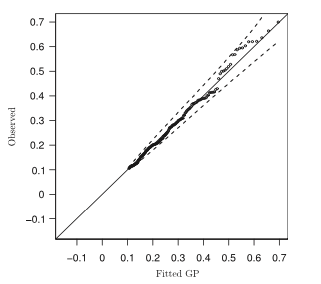
\includegraphics[width=2.0in]{project/papafiles/fig8.papa.gp.png}}
{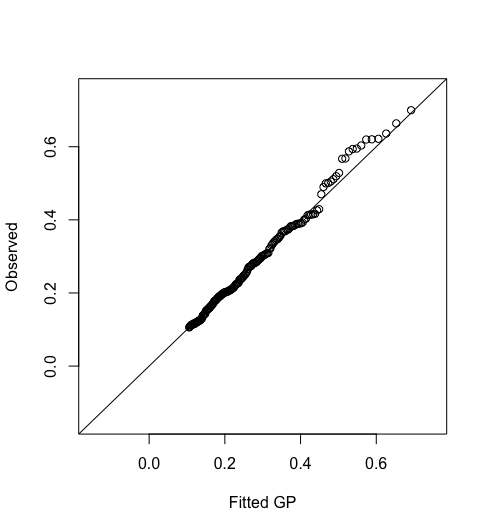
\includegraphics[width=2.0in]{project/papafiles/fig8.me.gp.png}}
\caption{QQ plot for diagnosis of GP fit of data above 70\% quantile. Left: \cite{papatawn}, right: reproduction }
\end{center}
\end{figure}

\section{Application to Precipitation data - Rain}
Following the reproduction of experiments from \cite{papatawn}, an investigation on the efficacy of EGPs on new data was conducted. This analysis follows steps similar to those outlined in section 5. The data consists of the Summer (May to August) rain data around the Toronto international airport collected between 2015 and 2020 \footnote{ \texttt{https://climate.weather.gc.ca/historical\_data/search\_historic\_data\_e.html}} and can be seen in Fig. 15.

\begin{figure}[H]
\begin{center}
{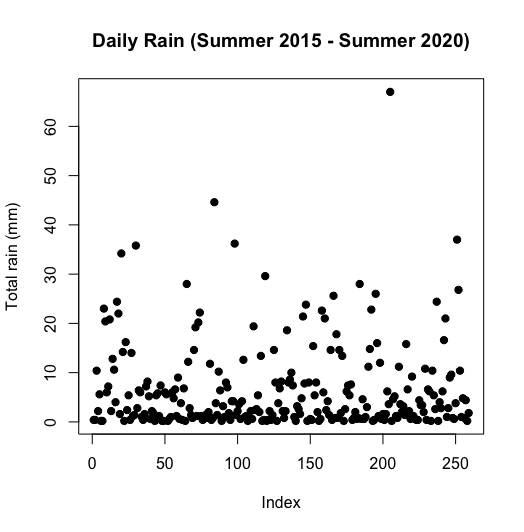
\includegraphics[width=3.0in]{project/papafiles/rain.png}}
\caption{Rain data from Summer 2015 to Summer 2020 around Toronto international airport.}
\end{center}
\end{figure}

Using this data, grid of 30 evenly spaced thresholds from the 0\% quantile (0.2) to the 80\% quantile (10.68) is formed. Both the EGP1 and GP models are fit over this range of thresholds. The experiment investigates the parameter stability, model diagnostics, and return level stability from the fit of both an EGP1 and a GP.

\subsection{Parameter Stability}
Fig. 16 depicts the stability plot featuring the estimated parameters. Using the stability of the modified scale as criterion, 0.2 (entire data) and 1.64 are chosen as thresholds for the EGP1 and GP models respectively. From this figure, it is apparent that the GP parameters behave in a more stable fashion than the EGP1 parameters.

\begin{figure}[H]
\begin{center}
{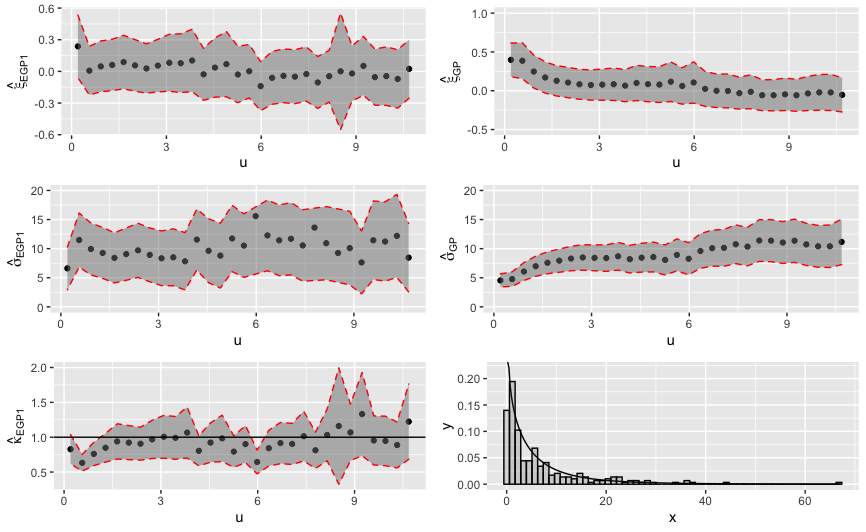
\includegraphics[width=4.5in]{project/papafiles/rain.stab.png}}
\caption{Parameter stability plots from (left) EGP1 fit and (right) GP fit. The bottom right shows histogram of rain data along with estimated density from the EGP1 model fitted to exceedences above 0.2 mm.}
\end{center}
\end{figure}
Though the stability plot favours the use of GP over EGP1, we may still use the EGP1 model as a diagnostic for the GP. In fact, we observe that the minimum value for which $\hat \kappa$ close to 1 corresponds exactly to the minimum threshold after which the modified scale (as estimated by GP) stabilizes. This observation is supported by the correspondence between EGPs and GP models.

\subsection{Model diagnostics}
In Fig. 17, the advantages of the EGP model over the GP model are evident. The EGP1 model better estimates the upper tails of our data than the standard GP model. This is crucial in the next section as the return level stability plots may now be considered relative to the model diagnostic plots.
\begin{figure}[H]
\begin{center}
{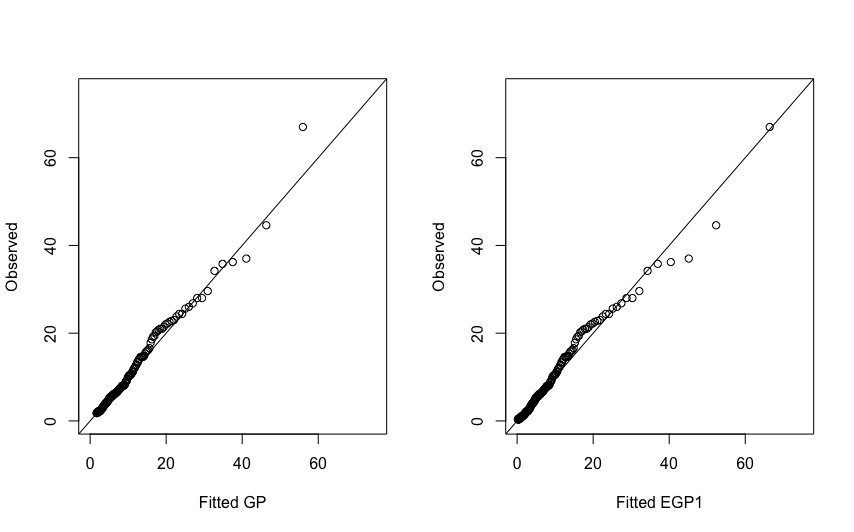
\includegraphics[width=3.in]{project/papafiles/rain.qq.png}}
\caption{QQ diagnostic plot from fit of GP (left) with threshold of 1.65 and EGP1(right) with threshold of 0.2}
\end{center}
\end{figure}

\subsection{Return Level Stability}
Next, the behaviour of the estimated return levels from EGP1 and GP models is examined. Seven equally spaced thresholds between the 0\% quantile (0.2) and the 90\% quantile (19.56) of the data are chosen. For each of these, the 10, 50 , 100, 200, and 500 observation return levels are estimated. Fig. 18 illustrates the estimates for these return levels. 
\begin{figure}[H]
\begin{center}
{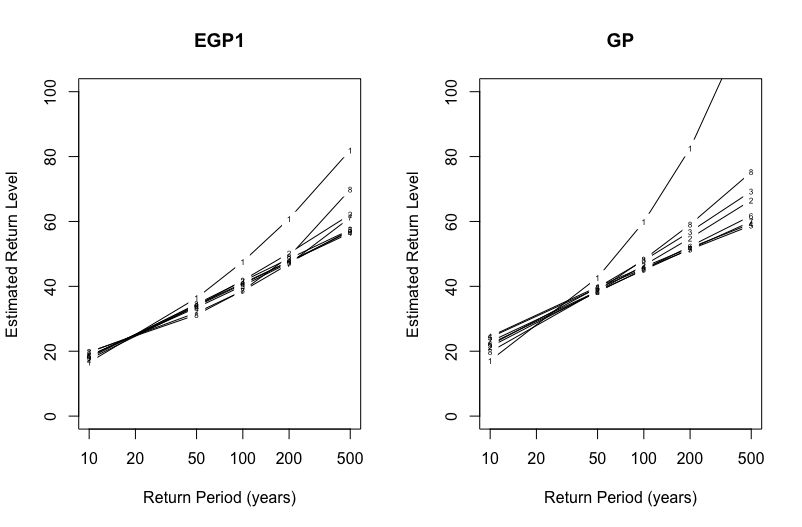
\includegraphics[width=4.in]{project/papafiles/rain.return.png}}
\caption{ Estimates of 10-, 50-, 100-, 200- and 500-observation return level obtained from fitted EGP1 (left) and GP (right) above range of thresholds 0.2 to 19.65 encoded by numbers 1-8. }
\end{center}
\end{figure}
From the figure above, it can be assumed inference made on EGP1 models would yield more stable results than those made from the GP. In fact, return levels from the EGP1 model seem to decrease as the thresholds increases. In contrast, the return levels from the GP model appear to have no discernible basis for their ordering.

\section{Conclusions}

\cite{papatawn}

\bibliographystyle{plain}
\bibliography{refs}
\end{document}